\subsection{Indkøbsliste}
En indkøbsliste kommer til verdenen ved at man i husstanden beslutter sig for at benytte en indkøbsliste. Dette kan være i form af et papir der ligger et fast sted på bordet eller hænger på opslagstavlen. Denne hændelse kaldes \textit{indkøbsliste oprettet}. Så længe den ligger der på bordet eller et andet sted, kan mange personer komme forbi og tilføje eller fjerne ting på den. Denne tilstand kaldes for \textit{redigeres}. I denne tilstand er det muligt at tilføje ingredienser fra en opskrift man mangler ingrediensen for at lave. Man kan også fjerne en ingrediens ved at slå en streg over den, og give et klart signal om at denne ikke skal købes. Disse to hændelser hedder \textit{ingrediens tilføjet} og \textit{ingrediens fjernet}. Man kan også skrive andre ting på en indkøbsliste end ingredienser. Det kan være en bemærkning, \fx ``hvis det er på tilbud''. Denne bemærkning kan selvfølgelig også fjerne igen på samme måde som en ingrediens. Disse to hændelser hedder \textit{tekst tilføjet} og \textit{tekst fjernet}. Når en person beslutter sig for at tage indkøbslisten med på indkøb, anses indkøbslisten for at være færdig. Denne hændelse kaldes \textit{indkøbsliste færdig}. Hele husstanden har altså ikke mulighed for at redigere denne mere, og indkøbslisten får derfor tilstanden \textit{aktiv}. Ude i supermarkedet kan man købe mange forskellige råvarer. Dette overvåges med hændelsen \textit{råvare købt}. Det bør bemærkes, at indkøbslisten indeholder ingredienser, hvilke består af en råvare, en mængde og en enhed. Vi ønsker ikke at overvåge hvor meget folk har af en ingrediens, og benytter derfor istedet objektet råvare, der ikke indeholder nogen mængde eller enhed. Denne beslutning er taget på baggrund af møde 2 med vores informanter. 
\begin{figure}[htp]
\centering
\scalebox{0.6}{
\subsection{Indkøbsliste}
\label{subsec:brug-indkoebsliste}

Ud over muligheden for at tilføje opskrifternes ingredienser til indkøbslisten, så kan man også tilføje almindelig tekst til, så det er muligt at lave en indkøbsliste, der indeholder andet end ingredienser til madlavningen. Så man kan skrive andre varer på, som man kan købe med fra \fx supermarkedet. Systemets indkøbsliste kan ses i \figref{fig:overblik-indkoebsliste}.

\begin{figure}[H]
	\centering
	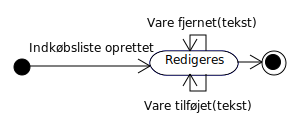
\includegraphics[scale=1]{billeder/foodl/thumbnails/indkoebsliste.png}
	\capt{Denne figur har til formål at give et overblik over systemets indkøbsliste.}
	\label{fig:overblik-indkoebsliste}
\end{figure}

Brugeren har mulighed for at tilføje varer i feltet ``tilføj til indkøbsliste'' og trykke på ``tilføj'' i bunden af siden. Der er mulighed for at slette alle varer fra indkøbslisten, ved at trykke på knappen ``slet alt'' i øverste højre hjørne af indkøbslisten, og ligeledes at slette enkelte varer, ved at trykke på de små gule krydser ud for alle varerne. Derudover er der implementeret en knap, til at udskrive indkøbslisten, som vi naturligvis kalder for ``udskriv''.

Hvis brugeren ikke er logget ind, vil de se i øverste højre hjørne af \figref{fig:overblik-indkoebsliste} (under sidehovedet) en boks, som informerer brugeren om, at man skal være logget ind for at systemet skal være i stand til at gemme indkøbslisten og favoritter. Oprettelse af bruger og indlogning bliver beskrevet nærmere i \secref{subsec:brug-opret}.
}
\capt{Tilstandsdiagram for Indkøbsliste-klassens adfærdsmønstre}\label{fig:indkoebsliste-adfaerd}
\end{figure}